\chapter{Literature review.}

The purpose of this review is to summarise the literature on currently available multi-objective reinforcement learning algorithms. Section 1 of this chapter is an introduction to single objective reinforcement learning including common terms, definitions and notation. The second section is devoted to the multi-objective optimization and its influence on multi-objective reinforcement learning. Finally, Section 3 is a literature review of the important papers in multi-objective reinforcement learning.

\section{Elements of reinforcement learning}
Multi-objective reinforcement learning is a direct extension from single objective reinforcement learning. Both these disciplines share much of the same notation and terminology.

This section will introduce the core concepts of reinforcement learning in the context of a single objective function. The extension of these concepts to multiple objectives will be addressed in section 1.3.

\subsection{The Problem.}

Consider a multi-step decision making process with unknown reward and state transition functions. We can look at this process as an optimization problem in which the aim is to make the correct decision at each step in order to maximize some measure of the rewards received. Any method that solves this optimization problem can be defined as a reinforcement learning method.

\subsection{Agent and environment}
\label{sec:agent-and-environment}

A reinforcement learning problem can be further divided into two parts: an agent and an environment. The agent or so called decision maker or a learning algorithm is responsible for actions at each time step. The actions chosen by the agent affect the environment and cause it to transition from one state to another. This dynamic interaction constitutes the agent-environment cycle shown in Figure~\ref{fig:agent-env-cycle}.

\begin{figure}[ht]
\vskip 0.2in
\centering
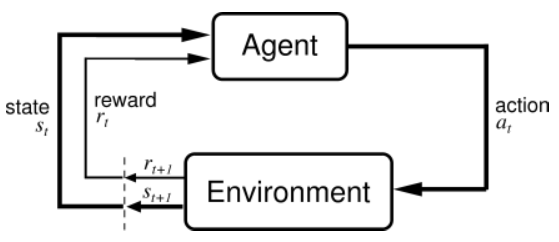
\includegraphics[scale=0.9]{agent-env-cycle.png}
\caption{The agent-environment cycle (Sutton and Barto, 1998).}
\vskip -0.2in
\label{fig:agent-env-cycle}
\end{figure}

The agent interacts with the environment with the help of three signals: a state signal, which describes the current state of the environment; an action signal, by which the agent interacts with the environment and a scalar reward signal, a feedback from the environment on the desirability of the immediate consequences of the action. At each time step of the agent-environment cycle, the agent senses the current state of the environment and applies an action. This action causes the environment to transition into a new state. After each state transition a reward (possibly zero) is passed to the agent. This reward evaluates the quality of the taken action. Along with the reward the agent senses the new environmental state. This process happens at each time step. The agent does not control state transitions and reward received. Instead the transition function and a reward function along with the set of possible actions and the set of all possible states belong to the environment which is often assumed to be a Markov decision process (MDP) (Bertsekas, 1995\nocite{bertsekas1995dynamic}). \\

Mathematically speaking a MDP consists of 2 sets and 2 functions. The two sets are the set of all possible states $\textit{S}$ and a set of all possible actions $\textit{A}$. The two functions are the transition function $\emph{f}$ and the reward function $\rho$. During interaction between the agent and the environment transition function $\emph{f}$ changes the state of the environment in response to the action signal. Right after state transition the reward function $\rho$ produces a scalar reward signal, i.e. immediate reward for an agent. During a time step $\emph{t}$ the agent applies action $\emph{$a_{t}$}$ in the state $\emph{$s_{t}$}$. The state changes to $\emph{$s_{t+1}$}$ according to the transition function $ f : S \times A \rightarrow S $:

$$\emph{$s_{t+1}$} = \emph{f}(\emph{$s_{t}$},\emph{$a_{t}$})$$

And the agent receives the scalar reward $\emph{$r_{t+1}$}$, according to the reward function $\rho$ : $\emph{S}$ $\times$ $\emph{A}$ $\rightarrow$ $\mathbb{R}$:

$$\emph{$r_{t+1}$} = \rho(\emph{$s_{t}$},\emph{$a_{t}$})$$

It is important to notice that both functions $f$ and $\rho$ can be either deterministic or stochastic.

The agent chooses actions according to its policy. The policy manifests which actions to pick at particular states $\pi$ : $\emph{S}$ $\rightarrow$ $\emph{A}$ :

$$\emph{$a_{t}$} = \pi(\emph{$s_{t}$})$$

Because environment is represented as a Markov decision process, it has the Markov property. That is given only $\rho$, $\emph{f}$, $\emph{$a_{t}$}$, $\emph{$s_{t}$}$ it is possible to determine the probability distributions of $\emph{$s_{t+1}$}$ and $\emph{$r_{t+1}$}$. This implies that all of the information required to make optimal decisions is contained within the current state vector $s_{t}$ - the agent need not take into account any historical information about previous states and actions. A good example is the chess game. One doesn't need to know the previous moves to decide the current move. It is enough to know the current positions of all figures on a board to make a decision.


\subsection{Agent's goals.}
On every stage of the decision process an agent chooses an action. The quality of the chosen action is evaluated and a reward is returned to the agent. This setting allows us to formalize the goal of the agent. The goal of the agent is an optimization problem of maximizing the amount of rewards throughout a course of interaction between agent and envrionment . In other words the agent must decide which sequence of actions will result in maximum of the rewards.

This formalization of the goal naturally reflects the learning process found in people and animals and thus allows to model many of the problems found in real life.

A \textit{return} is a cumulative sum of rewards obtained by the agent starting at some state $s_{0}$
$$\gamma^{0}\textit{r}_{1}+\gamma^{1}\textit{r}_{2}+\gamma^{2}\textit{r}_{3}+...$$

Here, the discount factor $\gamma$ $\in$ [0,1). First, this $\gamma$ guarantees convergence over the infinite horizon and second it denotes that the agent gives more weight to immediate rewards rather than delayed rewards.

Alternatively the return could be written like this:

$$ \emph{$R^{\pi}$}(s_{0}) = \sum_{t=0}^{\infty}\emph{$\gamma^{t}r_{t+1}$} = \sum_{t=0}^{\infty}\emph{$\gamma^{t}\rho$}(\emph{$s_{t}$},\emph{$\pi$}(\emph{$s_{t}$})). $$

And again $\gamma$ is the discount factor and $\emph{$s_{t+1}$}$ = $\emph{f}$ ($\emph{$s_{t}$}$,$\emph{$\pi$}$($\emph{$s_{t}$}$)) for $\emph{t}$ $\geq$ 0 and $\emph{$\pi$}$ is the policy being used.

Essentially, $ \gamma $ converts an infinite horizon MDP into a finite one. It is important to notice that in some cases it is possible to remove $ \gamma $ completely. For example, consider a case of a finite MDP with a -1 penalty for each move of an agent. In this setting this penalty will essentially work as $\gamma$.

\subsection{Dynamic Programming influence.}

Dynamic programming (Bellman, 1956\nocite{bellman1956dynamic}) is the scientific discipline centered around calculating the optimal policies for a given MDP. It has a strong assumption that we have a perfect model of the MDP (full knowledge of the transition and the reward functions).

Reinforcement learning has a strong connection to the dynamic programming. As was said before the dynamic programming requires the knowledge of both transition and reward functions. But in some scenarios this information is not available to us. Cases like these are the natural application of the reinforcement learning. The following paragraphs will describe terms that are common to both the dynamic programming and the reinforcement learning.

\subsubsection{Value Functions and Bellman Equation.}

A large optimization problem of maximizing a reward over all stages can be broken into a sequence of smaller problems. Each of these small problems is centered around picking an action which will maximize the combination of the immediate reward and a cumulative sum of rewards that follows the next state of the environment. This requires us to have some means to store and access the cumulative reward associated with each state of an environment.

A \textit{Value function} is a function that takes a state (or a combination of a state and an action) and returns the expected future reward that follows that state (or state-action). In essence, a value function describes the "goodness" or value of visiting a state and allows the agent to compare states with each other.

The value of a state $s_{t}$, at time step $t$, depends on the rewards $ r_{t+1},r_{t+2},... $. Which in turn depend on actions being taken at time steps $ t, t+1,... $. Actions of course depend on a policy being used by a decision-maker. Thus a value function of a state $s$ is denoted $V^{\pi}(s)$, with regard to some policy $\pi$, which underlies a decision making process.

Formally we can write
$$ V^{\pi}(s)=E_{\pi}\{R_{t}\;|\;s_{t}=s\} = E_{\pi}\left\{\displaystyle\sum_{k=0}^{\infty}\gamma^{k}r_{t+k+1}\;|\;s_{t}=s\right\}. $$

Function $V^{\pi}$ is called the \textit{state-value function} for policy $\pi$. The state-value functions are good for conveying the theory of multi-step decision processes. In practice, however, they are replaced by so called \textit{action-value functions}. The action-value function estimates the value of not only visiting a state $s$ but also of taking some action $a$ at that state, and subsequently following a policy $ \pi $. Formally we can write
$$ Q^{\pi}(s,a)=E_{\pi}\{R_{t}\;|\;s_{t}=s,a_{t}=a\} = E_{\pi}\left\{\displaystyle\sum_{k=0}^{\infty}\gamma^{k}r_{t+k+1}\;|\;s_{t}=s,a_{t}=a\right\}. $$

We can further notice that
$$ V^{\pi}(s)=E_{\pi}\{R_{t}\;|\;s_{t}=s\} $$
$$ =E_{\pi}\left\{\displaystyle\sum_{k=0}^{\infty}\gamma^{k}r_{t+k+1}\;|\;s_{t}=s\right\} $$
$$ =E_{\pi}\left\{r_{t+1}+\gamma\displaystyle\sum_{k=0}^{\infty}\gamma^{k}r_{t+k+2}\;|\;s_{t}=s\right\} $$
$$ =E_{\pi}\{r_{t+1} + \gamma V^{\pi}(s_{t+1})\;|\;s_{t}=s\}. $$

This equation is called the \textit{Bellman equation} for $ V^{\pi} $. The Bellman equation describes the connection between the value of a current state and the values of possible successor states. This fundamental recursive  relationship forms the foundation for a number of techniques to estimate correct values for $V^{\pi}$.

\subsubsection{Optimal Value Functions.}

Value functions allow us to compare different policies with each other, and naturally (because we are working with finite MDPs) there will be at least one best policy. To illustrate this we can visualize the given MDP as a tree. The tree's root is a starting state. Each branch of the tree represents a sequence of decisions (a policy) and the corresponding rewards. When the tree is finite there are a finite sequence of scalar rewards corresponding to each branch of the tree. One of those sequences will be the maximum. We can still apply the same logic even if the given MDP is infinite. In fact this is one of the reasons for using the discounting factor in the definition of return. The discounting factor allows us to represent the infinite MDP as the finite tree of decisions. We define a policy $\pi$ to be better than a policy $\pi'$ if it achieves higher or equal expected return for all states $s \in S $. Designation for optimal policy is $ \pi^{*} $.

Any policy leads to a value function and naturally the optimal policy $ \pi^{*} $ leads to the optimal value function $ V^{*} $. Formally we define $ V^{*} $ as

$$ V^{*}(s) = \max_{\pi}V^{\pi}(s), \;\;\;\;\text{for all}\; s \in S. $$

Now we can reformulate the reinforcement learning problem as finding the optimal policy $ \pi^{*} $ and associated optimal value function $ V^{*} $.

\subsubsection{Value Iteration.}

We now turn to how estimate the optimal policy. One particular algorithm is called \textit{value iteration}. This is an iterative algorithm which starts with any randomly initialized value function $V_{0}$. With each iteration $k$, the algorithm produces an approximation $V_{k}$, until it converges to the optimal value function $V^{*}$.

The value function is updated according to the following update rule:

$$ V_{k+1}(s) = \max_{a}\displaystyle\sum_{s'}T(s,a,s')\;[R(s,a,s')+\gamma V_{k}(s')], \;\;\;\;\text{for all}\; s \in S, $$
where $ T(s,a,s') $ is the probability to transition to the state $s'$ given state $s$ and action $a$, and $ R(s,a,s') $ is the immediate reward for transition to the state $s'$ given state $s$ and action $a$.

Here index $k$ can be viewed as the number of future rewards ahead that we are taking into account. For example, $k=0$ means that we are considering 0 time steps ahead, meaning that we are not considering even immediate reward.

\subsubsection{Policy Iteration.}

One of the disadvantages of the value iteration algorithm is due to the stopping criteria of the algorithm. In order to find whether we should stop the algorithm we need to observe the values for iterations $k$ and $k+1$. We can stop the algorithm only when we have a significant evidence that the values for all states are no longer improving. This gives rise to the situation when the optimal action for each state is already identifiable but there is still some difference between $ V_{k} $ and $ V_{k+1} $, for example due to small learning rate. Thus the algorithm may spend unnecessary amount of time just to meet formal criteria of convergence.

The algorithm called \textit{policy iteration} (Bellman, 1956\nocite{bellman1956dynamic}) is able to address this particular problem. The first step of the policy iteration algorithm is called the \textit{policy evaluation} (Bellman, 1956\nocite{bellman1956dynamic}). During the policy evaluation step, the algorithm is given any intermediate policy $ \pi_{i} $. This policy is then evaluated using the following update rule:

$$ V_{k+1}^{\pi_{i}}(s) = \displaystyle\sum_{s'}T(s,\pi_{i}(s),s')\;[R(s,\pi_{i}(s),s')+\gamma V_{k}^{\pi_{i}}(s')], \;\;\;\;\text{for all}\; s \in S, $$
where $ T(s,\pi_{i}(s),s') $ is the probability of transition to the state $s'$ given state $s$ and action $ \pi_{i}(s) $, and $ R(s,\pi_{i}(s),s') $ is the immediate reward for transition to the state $s'$ given state $s$ and action $\pi_{i}(s)$.

The policy evaluation step has a lot of similarities with the value iteration algorithm. Only in the policy evaluation we are not looking for a maximum over all possible actions and we are using a fixed policy $ \pi_{i} $.

Once the policy evaluation has converged, we proceed to the \textit{policy improvement} (Bellman, 1956\nocite{bellman1956dynamic}) step. We update the intermediate policy $ \pi_{i} $ according to the following rule:
$$ \pi_{i+1}(s) = \arg\max_{a}\displaystyle\sum_{s'}T(s,a,s')\;[R(s,a,s')+\gamma V_{k}^{\pi_{i}}(s')], \;\;\;\;\text{for all}\; s \in S, $$
where $ T(s,a,s') $ is the probability to transition to the state $s'$ given state $s$ and action $a$, and $ R(s,a,s') $ is the immediate reward for transition to the state $s'$ given state $s$ and action $a$.

The stopping criteria for the policy iteration is reached when we no longer able to improve intermediate policy $ \pi_{i} $ and thus we declare $ \pi_{i} $ to be the optimal policy $\pi^{*}$.

The advantage of the policy iteration over the value iteration lies within the policy evaluation update rule. This update rule doesn't have the maximum over all action operator $(\max_{a})$, since the policy under evaluation is fixed; This gives a significant speed of convergence advantage.

\subsubsection{Utility Functions.}
Dynamic programming aims to find an optimal sequence of decisions from any state $s$ given an MDP. This task involves considering each possible sequence of decisions (each outcome) from the state $s$ and deciding which of the outcomes is more preferable; Utility function in an MDP is the function which takes as an argument a sequence of actions and assigns a real-valued number which designates the utility of this sequence. Normally, the utility function will add all immediate rewards generated by the sequence of actions, representing a cumulative return.
 
In dynamic programming, given a sequence of immediate rewards $[r_{0},r_{1},r_{2},...]$, there are two ways to calculate the utility of this sequence:
\begin{enumerate}
  \item additive utility - $U([r_{0},r_{1},r_{2},...])=r_{0}+r_{1}+r_{2}+...\;$. 
  \item discounted utility - $U([r_{0},r_{1},r_{2},...])=r_{0}+\gamma r_{1}+\gamma^{2} r_{2}+...\;$.
\end{enumerate}
The first one is normally used in finite MDPs and the second one is used in infinite MDPs (to make sure that the cumulative return will not grow infinitely). 

Additive utility function implies that preferences over sequences of actions are stationary\footnote{This fact is very important as all methods for solving the Bellman optimality equation assume that preferences are stationary.}. Given two sequences of rewards $[a_{0},a_{1},...]$ and $[b_{0},b_{1},...]$ such that
$$ [a_{0},a_{1},...] \succ [b_{0},b_{1},...], $$
where the symbol $\succ$ means is more preferable. This preference is stationary if and only if
$$ [a_{0},a_{1},...] \succ [b_{0},b_{1},...] $$
$$ \Updownarrow $$
$$ [r,a_{0},a_{1},...] \succ [r,b_{0},b_{1},...]. $$
That is if the sequence $[a_{0},a_{1},...]$ is preferable over the sequence $[b_{0},b_{1},...]$ then it should stay preferable one or more steps in the future.

\subsection{Q-Learning.}
\label{sec:q-learning}
Policy iteration does not directly translate to the realms of the reinforcement learning as it requires the knowledge of a model of an environment (knowledge of reward and transition functions). Look at the update rule for the policy evaluation:
$$ V_{k+1}^{\pi_{i}}(s) = \displaystyle\sum_{s'}T(s,\pi_{i}(s),s')\;[R(s,\pi_{i}(s),s')+\gamma V_{k}^{\pi_{i}}(s')]. $$
And the update rule for the policy improvement:
$$ \pi_{i+1}(s) = \arg\max_{a}\displaystyle\sum_{s'}T(s,a,s')\;[R(s,a,s')+\gamma V_{k}^{\pi_{i}}(s')]. $$
They both require the knowledge of the functions $T$ and $R$, where $T$ is a state-transition function and $R$ is a reward function.

Reinforcement learning equivalent of policy iteration is called \textit{Q-Learning} (Watkins, 1992\nocite{watkins1992q}). Q-Learning, like DP value iteration, makes sure that any randomly initialized Q function converges to optimal action-value function $Q^{*}$. See Algorithm~\ref{alg:q-learning} for details.
\begin{algorithm}[tb]
   \caption{Q-Learning}
   \label{alg:q-learning}
\begin{algorithmic}
   \STATE {\bfseries Input:} Initialize $Q(s,a)$ randomly
   \REPEAT
       \STATE Initialize starting state $s$
       \REPEAT
           \STATE Choose $a$ from $s$ using policy derived from $Q$
           \STATE Take action $a$, observe $r$, $s'$
           \STATE $Q(s,a) \leftarrow Q(s,a) + \alpha [r + \gamma\; max_{a'}Q(s',a') - Q(s,a)] $
           \STATE $ s \leftarrow s'$
       \UNTIL{$s$ is terminal}
   \UNTIL{no more episodes}
\end{algorithmic}
\end{algorithm}
Q-Learning is a temporal-difference learning algorithm (Sutton and Barto, 1990\nocite{Sutton90time-derivativemodels}). The value iteration algorithm uses an expected value operator which requires knowledge of the state-transition function. Temporal-difference learning algorithms work around this by modifying update rule to work with raw experience. The update rule is slightly modified but essentially it does the same job only without the expected value operator:

$$ Q(s_{t},a_{t}) \leftarrow Q(s_{t},a_{t}) + \alpha \; \left[\;r_{t+1} + \gamma\; \max_{a}Q(s_{t+1},a) - Q(s_{t},a_{t})\;\right]. $$

Q-Learning requires several criteria to be met:
\begin{itemize}
  \item Underlying problem must be a Markov Decision Process.
  \item Learning rate $ \alpha $ should decrease to zero.
  \item Every state-action pair should be tried infinitely many times.
\end{itemize}
However, in practice the algorithm converges without some of these strict criteria. For example, in many cases the algorithm is able to converge with fixed $ \alpha $ parameter.

\subsection{Off-policy and On-policy algorithms.}
Previous section noted that temporal-difference methods such as the Q-Learning must be built in a way that ensures that every state-action pair is visited infinitely many times. This criterium is essential from the convergence point of view, remember that in the reinforcement learning a reward function is unknown to a learning algorithm and the only way to find the optimum sequence of actions is to try them all and calculate which one produces higher return. This means that the learning algorithm must at some point ignore a greedy action suggested by his current approximation of an optimal value function and instead choose some other action hoping that it will lead to a higher return.

One can run a series of episodes starting from the same starting state and record the return in each of the episodes. The average of those returns may differ from the value of the starting state predicted by the learned optimal Q-function. That is there will be a difference between the learned optimal Q-function and the actual results while the agent is learning. This behaviour is due to:
\begin{itemize}
  \item Q-learning learns the value of optimal sequence of actions given any starting state.
  \item The algorithm will introduce a randomness into action-selection process to insure that every state-action pair is selected (required by proof of convergence). Thus the actual sequence of actions taken by the agent will almost never be optimal.
\end{itemize}

Off-policy algorithms, such as Q-learning, do not record the actual value of each state-action pair, rather they record optimal value; They miss the fact that during each action-selection phase there might be a random action with potential negative outcome. As a result the agent might easily identify the greediest action among available actions but it will miss the fact that taking that greedy action might potentially result in big penalties due to possible exploratory actions.

On the other hand, on-policy methods do take into account the randomness associated with the action selection mechanism of the policy being followed. Thus the values $ Q_{\pi}(s,a) $, for each state action pair, reflect the average of all sequences of actions that are possible under the policy $ \pi $.

Q-learning is ideal for applications where an identification of optimal policy is the only goal. That is when there is no harm done to the agent itself or other involved parties if the agent has performed an action which results in big penalties. An example is escaping from a maze - the goal is to find an optimal escape route. It doesn't matter how many times the agent was circling around the maze while exploring. On the other hand, if a Mars rover is exploring the surface of the planet, it becomes very expensive and potentially dangerous for the equipment.



\subsection{SARSA.}

Sarsa is a temporal-difference algorithm similar to Q-learning, except it is an on-policy method. Both algorithms are very similar; The only difference is the update rule employed in each of the algorithms. The Q-learning has the following update rule:

$$ Q(s,a) \leftarrow Q(s,a) + \alpha [r + \gamma\; max_{a'}Q(s',a') - Q(s,a)]. $$

Here the construct $ max_{a'}Q(s',a') $ reflects the fact that only the greediest path from successor state $ s' $ is taken into account while updating the state-action pair $ Q(s,a) $.

The Sarsa algorithm has the following update rule:
$$ Q(s,a) \leftarrow Q(s,a) + \alpha [r + \gamma\; Q(s',a') - Q(s,a)]. $$

Sarsa doesn't try to maximize the value with which to update $ Q(s,a) $. Instead,  $ Q(s',a') $ is the return from successor state after taking action $ a' $, which was selected according to the policy being followed by the agent.

\section{Multi-objective Optimization.}

Multi-objective reinforcement learning methods are built upon methods from general multi-objective optimization. Therefore this section will briefly describe the main concepts and techniques that were borrowed from general multi-objective optimization.

\subsection{Multi-objective Problem.}

Let $A$ be a set of all possible actions. Given $n$ objective functions $ f_{1}(),...,f_{n}() $ , we map each action $a$ from the set $A$ to a point $ (f_{1}(a),...,f_{n}(a)) $ in the $n-$dimensional objective space.

Multi-objective problem is the problem of finding actions $a$ from the set $A$ such that we are most satisfied with the reward vectors $ (f_{1}(a),...,f_{n}(a)) $.

\subsection{Tradeoffs.}

Multi-objective optimization aims to solve difficult real life problems and many of these problems involve objectives that conflict with each other. Introduction of these conflicting objectives means that in many cases we will not have a single best option. Or in other words we cannot improve all objective functions at the same time. Rather we will need to compromise between two or more objectives, gaining more value on one objective at the expense of the other(s).

\subsection{Dominance.}
\label{sec:dominance}
Given two solutions $a'$ and $a''$ we can map them into two points in the $n$-dimensional objective space:
$$ x'=(x'_{1},...,x'_{n}) \;\;\;\;\text{and}\;\;\;\; x''=(x''_{1},...,x''_{n})$$
where
$$ x'_{i} = f_{i}(a') \;\;\;\;\text{and}\;\;\;\; x''_{i} = f_{i}(a'') \;\;\;\;\text{for}\;\;\;\; i = 1,...,n $$
The point $x'$ is said to Pareto dominate (Pareto, 1896\nocite{pareto1896cours}) point $x''$ when
$$ x'_{i} \geq x''_{i} \;\;\;\;\text{for all}\; i, $$
and
$$ x'_{i} > x''_{i} \;\;\;\;\text{for at least one}\; i.\footnote{For consistency with reinforcement learning discussion it will be assumed that the agent's objective is to maximize the objective functions, whereas in most multi-objective optimization literature the goal is to minimize the objectives. In fact, the two cases are fundamentally equivalent.} $$

Dominated points by definition will imply the existence of solutions that achieve more on each of the objectives and because our goal is to maximize the objective function we may omit dominated solutions. On the other hand, we may find two solutions which outperform each other on one of the objectives. In this case we really cannot say which solution is better, since each of them excels on one of the objectives. We call them non-comparable solutions. The set of all non-comparable solutions constitutes the Pareto front (Pareto, 1896\nocite{pareto1896cours}).

\subsection{The Pareto Front.}

Every action $a$ in the actions space $A$ is getting mapped to a point $ (f_{1}(a),...,f_{n}(a)) $. The image of the set $A$ in the $n$-dimensional objective space is called $the\; range \;set\; R$. The subset of $R$ which consists of non-dominated solutions is called $the\; Pareto\;front$, as shown in Figure~\ref{fig:paretoFront}.

Now we can reformulate multi-objective problem as the problem of locating any of the points belonging to the Pareto Front. Which point should it be? All of the points are not comparable to each other. If the tradeoff is a matter of a personal preferences then a personal opinion is required to make a decision.
\begin{figure}[ht]
\vskip 0.2in
\centering
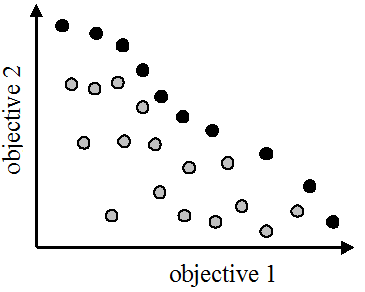
\includegraphics[scale=0.9]{paretofront.png}
\caption{The Pareto front is represented with black points. Each black point is a non-dominated solution. Grey points represent dominated solutions. Each gray point is dominated by at least one black point.}
\vskip -0.2in
\label{fig:paretoFront}
\end{figure}


\subsection{Selecting a Solution in The Pareto Front.}
\label{sec:Selecting-a-solution-in-the-Pareto-Front}
To reach a point in the Pareto front we need a scalar index which will reflect the preference between any two points. We can introduce a function $v$ defined on the $range \;set\; R$ with the following property:
$$ v(x_{1},..., x_{n}) \geq v(y_{1},..., y_{n}) $$
if and only if the point $ (x_{1},..., x_{n}) $ is more preferable or equal to the point $ (y_{1},..., y_{n}) $.

The following two sections will briefly describe two techniques to introduce that function $v$. These techniques are used in a large portion of multi-objective reinforcement learning algorithms and thus deserve a mention.

\subsubsection{Linear-Weighted Averages.}
Assume as before that the existence of a solution set $A$ and we also have $n$ objective functions $ f_{1}(),...,f_{n}() $. Each solution $ a\in A $ is mapped to a point $ (f_{1}(a),...,f_{n}(a)) $. Let
$$ \textbf{w} = (w_{1},...,w_{n}) $$
be a weight vector. Where
$$ w_{i} > 0, \;\text{for all }\; i $$
and
$$ \displaystyle\sum_{i=1}^{n} w_{i} = 1. $$

Let us pose an additional optimization problem: choose $a \in A$ that will maximize
$$ \displaystyle\sum_{i=1}^{n} w_{i}f_{i}(a). $$

Assume solution $a^{*}$ maximizes this given optimization problem. Let $ \textbf{x} = (f_{1}(a^{*}),...,f_{n}(a^{*})) $, in the $n$-dimensional objective space, with solution $a^{*}$.

The claim is that this point \textbf{x} must belong to the Pareto optimal set. If this point was not a member of the Pareto front there must another point \textbf{y} which dominates point \textbf{x}. But it cannot be since it would imply
$$ \displaystyle\sum_{i=1}^{n} w_{i}y_{i} > \displaystyle\sum_{i=1}^{n} w_{i}x_{i} $$
And we already know that point \textbf{x} is the maximum of the given optimization problem.

The more weight we apply to the specified objective the more favourable to the specified objective will be the identified point of the Pareto front. This allows us to perceive weights as a form of preference. However, setting the preferences a priori means human interaction and sometimes it is not so clear how to set these preferences.

Another limitation of this approach is the inability to locate concave points of the Pareto front. For example if the Pareto front has a concave shape then this approach will only locate extreme points.

\subsubsection{Lexicographical Ordering.}
Another widely used approach is to order objective functions $ f_{1}(),...,f_{n}() $ according to their importance.

Given two solutions $a^{1}$ and $a^{2}$ we say that $a^{1}$ is better than $a^{2}$ when $$ f_{i}(a^{1}) = f_{i}(a^{2}), \;\;\;\;\text{for}\;\;\;\; i = 1,...,n-1$$
and
$$ f_{n}(a^{1}) > f_{n}(a^{2}). $$

This approach is intuitively easy to understand and in fact in many problems it is possible to clearly differentiate which objective is more important.

\section{Multi-objective Reinforcement Learning Research.}

Reinforcement learning initially was applied to find optimal policies in single objective problems. However, in recent years there has been a significant increase in the interest towards multi-objective reinforcement learning. This can be explained by the fact that sometimes it is just impossible to express a sophisticated problem in terms of just a single objective, and naturally this gave rise to multi-objective reinforcement learning. For further motivation refer to Roijers et al. (2013)\nocite{roijers2013survey}.

This section will review the main work done on temporal-difference multi-objective reinforcement learning. It is only a review of the most seminal works, for more details please refer to Roijers et al. (2013)\nocite{roijers2013survey}. The first subsection will review temporal-difference methods based on the linear scalarization while the second subsection will consider non-linear methods. This separation is selected partially because linear methods are proven to converge while non-linear may not.

\subsection{Multi-Objective Markov Decission Processes (MOMDP).}
As was mentioned in Section \ref{sec:agent-and-environment}, in Markov decision processes the quality of taking action $a$ in a state $s$ is evaluated via an immediate scalar reward signal $r$:
$$ r = \rho(s,a,s'), $$
where $s'$ is a successor state and $\rho()$ is a scalar reward function:
$$ \rho : S \times A \times  S \rightarrow \mathbb{R}. $$
In a MOMDP there are $n$ such reward functions $\rho_{1},\rho_{2},...,\rho_{n}$ and the immediate reward signal is a vector:
$$ \vec{r} = (\rho_{1}(s,a,s'),\rho_{2}(s,a,s'),...,\rho_{n}(s,a,s')). $$
This in turn makes the Q-function a vector-valued function:
$$ \overrightarrow{Q(s,a)} = (R_{1},R_{2},...,R_{n}), $$
where $R_{i}$ is the total cumulative return for an objective function $i$ if an agent decides to take an action $a$ in a state $s$.

Q-Learning, which was introduced in Section \ref{sec:q-learning}, was developed originally for single-objective MDPs, it can be observed from the update rule for this algorithm:
$$ Q(s_{t},a_{t}) \leftarrow Q(s_{t},a_{t}) + \alpha \; \left[\;r_{t+1} + \gamma\; \max_{a}Q(s_{t+1},a) - Q(s_{t},a_{t})\;\right]. $$
Here the maximization operator assumes that there is a clear ordering between available actions in state $s_{t+1}$ of an environment and in case of single objective MDPs this ordering is based on which action produces a higher scalar return. In contrast, in case of multi-objective MDPs it is no longer clear how to perform ordering of available actions as a Q-function for each action no longer produces a scalar number but rather a vector of values and those vectors may be non-comparable to each other (see Section \ref{sec:dominance}).

\subsection{Linear Temporal Difference Learning.}
Previous section pointed out that in order to make algorithms like the Q-Learning work in multi-objective MDPs some adjustments must be made to an update rule, namely there must be a clear mechanism which will resolve the ordering of available actions in some state $s$. One way to achieve this is through the use of a general multi-objective optimization technique called linear-weighted averages or simply linear scalarization (see Section \ref{sec:Selecting-a-solution-in-the-Pareto-Front}).

Given a multi-objective MDP, a policy $\pi$ and a $n$-component weight vector $\vec{w}$, a maximization operator based on the linear scalarization will compute a scalarized value for each available action $a$ in some state $s$ according to the following rule:
$$ \displaystyle\sum_{i=1}^{n} w_{i}Q^{\pi}_{i}(s,a), $$
where $n$ is the number of objectives in the MDP, $w_{i}$ is an $i$-th component of the weight vector $\vec{w}$ and $Q^{\pi}_{i}$ is an $i$-th component of a vector-valued Q-function under the policy $\pi$. The actions are ordered according to the scalarized value they produce.

Before linear scalarization was used in reinforcement learning, Feinberg and Shwartz (1993)\nocite{Feinberg93constrainedmarkov} wrote an extensive paper on using linear scalarization in constrained Markov decision models. The authors proved the existence of optimal policies in such models and also proved that linear scalarization is able to identify members of the Pareto front. Even though this paper didn't mention reinforcement learning, it provided the necessary theoretical foundations for other researchers to try out linear scalarization in multi-objective reinforcement learning.

Karlsson (1997)\nocite{Karlsson97learningto}, in his PhD thesis, first tried to combine Q-learning algorithm and linear scalarization. The author argues that when dealing with multi-criteria problem, it is much better to break a complex state space into a number of smaller state spaces, so called modules. For each module we maintain a separate Q-function. It helps to avoid relearning when dealing with a complex task consisting of a number of independent sub-tasks.

Having multiple separate Q-functions, Karlsson faced a problem of how to administer the action selection process. He used the so called "greatest mass method". To determine a value of some action under this method, one needs to sum this action's Q-values across all modules. An action with the greatest overall sum is pronounced the greedy action. Essentially, this method is just a linear scalarization with all weights equal to one.

The author provided details of his test environment, which he called the simple driving domain (SDD). The SDD is a grid world with roads crossing it vertically and horizontally. The world is populated with different objects: street signs, traffic lights and obstacles. An agent controls a car. The agent has four goals: stay on a road, avoid obstacles, negotiate streetlights, follow street signs. All tasks are independent of each other. The author specifically created independent sub-tasks to test the modular approach.

The main point of Karlsson's research was to investigate how agents behave when the complex state space is decomposed into smaller sub-spaces. For this purpose he also created one agent which maintained a complex structure of the state space (monolithic approach). His results show that in many scenarios the modular approach performs as well as monolithic approach, while having a significant advantage in terms of speed of convergence.

Castelleti et al. (2002)\nocite{castelletti2002reinforcement} further explored linear scalarization. They were interested in applying reinforcement learning methods to a water reservoir management. As a case study they chose Lake Como, which is located in Northern Italy. This lake provides water supply to agricultural districts and hydroelectrical power plants.

It is possible to model this problem as an MOMDP. State information includes: current water level and information about natural water income. Actions govern how much water to release from the reservoir. In this paper the authors used two objectives: provide water and avoid flooding.

Unlike the work of (1997)\nocite{Karlsson97learningto}, the researchers didn't break the complex state space into smaller ones. However essentially their approach is the same - to identify greedy actions, one combines Q-values of each objective into a weighted sum. Only in this case, weighted sum is no longer uniform and weights could be arbitrary (as long as they sum to 1). They called their algorithm Qlp (Q-Learning planning). The authors approximated the Pareto front by having multiple independent tests - each test for one weight set.

In the experimental results section the authors compared their proposed approach with the results obtained with the help of stochastic dynamic programming approach (SDP); The QLP consistently outperformed the SDP.

It is important to notice that it was probably the earliest work where non-uniform weights were used.

Natarajan and Tadepalli (2005)\nocite{natarajan2005dynamic} used linear scalarization to sequentially learn multiple optimal policies. All the papers discussed so far
organized trials in similar manner:

\begin{enumerate}
  \item Set preferences for each objective.
  \item Initialize value function.
  \item Learn optimal policy for a the specified set of weights.
\end{enumerate}

All these steps need to be performed when preferences are changed. The authors noticed that the learnt value function for previous set of weights can be used to speed-up the learning process. If sets of weights are significantly different then one will not observe noticeable improvements. On the other hand, if the preferences correspond to nearby points in the objective space then the learning process will take full advantage of the value function learnt before. The authors propose mechanism which allows to determine which of the previously learnt policies should be used when the preferences are changed.

Two experimental domains are included in the paper: modified Buridan’s ass problem and network routing problem. The modified Buridan’s ass is the modification of the original problem (G{\'a}bor et al., 1998\nocite{gabor1998multi}). The modified version has an increased state-space - 3 by 3 grid world. A donkey is located in the middle of the grid world and two plates of food are located in top-left corner and bottom-right corner of the world respectively. The donkey must reach either of the plates with food to stay alive but every time he reaches for one of the plates the one might be stolen. Oveall there are three objectives: amount of food eaten, number of plates stolen and a number of moves made by the donkey. The authors demonstrate experimental results, which show a significant reduction of time-steps needed to learn optimal policies when prior value functions.

The network routing domain represents typical computer network with a number of nodes connected though a specified network topology. Three objectives are present: end to end delay, number of packets lost and power consumed by a node. Each state is represented by a current node and destination node. Actions are represented by neighbors of the current node through which the packet might be sent. Overall goal is to find an optimal routing policy according to specified preferences. The experimental results again demonstrate that learning from scratch for each set of weights takes a significantly loner amount of time than learning from prior policies.\\

\subsection{Non-linear Temporal Difference Learning.}

In many applications there is a natural ordering of the objectives; For example, consider a cleaning robot with two objectives: maintain a battery charged at all times, and clean an office. In this scenario there is natural ordering - the battery of the robot should never deplete (cleaning is not possible if the robot's battery is depleted), thus maintaining the battery level is considered more important. Non-linear temporal-difference methods can accurately reflect this ordering of the objectives and thus are more suitable for this domain.

More importantly, it has been shown (Yaman et al., 2010\nocite{Yaman20111290}) that people often employ lexicographic ordering of the objectives while making complex decisions.

One of the most earliest and most widely cited publications in MORL is Gabor, Kalmar and Szepesvari (1998)\nocite{gabor1998multi}. The publication first develops a solution for multi-criteria dynamic programming. After that the solution is modified to be extended to multi-criteria reinforcement learning.

The authors aimed at developing a mechanism to order policies. For this purposes, they used a minimum threshold on one of the objectives. This allowed authors to use only one objective as a maximization criteria. This paper builds upon lexicographical ordering of objective functions, which was described in the the multi-objective optimization section (Section 1.2.5).

After showing that this approach converges for abstract multi-criteria dynamic programming problem, the authors extend the technique for multi-criteria reinforcement learning.

This publication goes to a great extent describing mathematical proof of the proposed algorithm. Apart from mathematical aspects, the authors also included experimental results. Using a game of tic-tac-toe, the authors were able to show that their algorithm was able to identify optimal policy. They used two objectives: to win a game and to do it as fast as possible.

Van Moffaert et al. (2012)\nocite{van2012scalarized} proposed to use Chebyshev scalarization function. They used Chebyshev distance in the process of evaluating a set of actions. To successfully use this distance the authors introduced a so called utopian point $z^{*}$ in the objective space. After applying scalarization function to any state-action combination $(s,a)$ we obtain a scalarized Q-value (SQ):
$$ SQ(s,a) = \max_{o=1...m} w_{o} \cdot | Q(s,a,o) - z^{*}_{o} | $$
, where $m$ is the number of objectives. Given any state $s$ and all available actions $a$, we define a greedy action to be a solution to the following optimization problem:
$$ \min_{a} SQ(s,a). $$

The authors tested their approach on two well studied multi-objective reinforcement learning problems: the Deep Sea Treasure and the multi-objective Mountain Car. They were able to demonstrate that on both problems their non-linear scalarization approach was able to locate more optimal polices than usual linear scalarization.

Van Moffaert et al. (2013)\nocite{van2013hypervolume} proposed to use hypervolume indicator to guide action selection process. Their action-selection strategy (algorithm~\ref{alg:hb-as}) drastically differs from both linear and non-linear scalarization methods.

The agent maintains a list $l$ of points in the objective space. The list $l$ is empty at the beginning of an episode. On every step of the episode we map selected state-action to the objective space, according to q-value of the state-action pair. The resulting point is added to the list $l$.

Given any state $s$ and some available action $a$, the proposed strategy maps this action to a point in the objective space. After that we add this point to the list $l$ and calculate the hypervolume. The action is called greedy when it has the biggest contribution to the hypervolume.

The list $l$ is empty at the beginning of an episode. On every step of the episode we map selected state-action to the objective space, according to q-value of the state-action pair. The resulting point is added to the list $l$.

This approach utilizes search in the objective space of a problem. That is the main difference from the methods based on the scalarization, where we take q-values for each objective and transform it to a single value. However, this algorithm also uses Q-learning as underlying learning mechanism.

\begin{algorithm}[tb]
   \caption{Hypervolume based action-selection}
   \label{alg:hb-as}
\begin{algorithmic}
   \STATE {\bfseries Input:} a state $s$, list $l$ of Q-values
   \STATE  $volumes \leftarrow \{\} $
   \FOR{ $\text{each action}\;a\; \text{available at given state}\;s$ }
       \STATE  $ \text{create m-component vector}\; \textbf{r} $
       \FOR{ $ \text{i = 0 to m} $ }
       \STATE  $ r_{i} \leftarrow Q(s,a)\; \text{ for objective}\;i  $
       \ENDFOR
       \STATE $ hv \leftarrow \textit{getHypverVolume( l} + \textbf{r} \textit{)} $  \STATE add $hv$ to $volumes$
   \ENDFOR
   \STATE \textbf{return} $ \argmax_{a}\; volumes $
\end{algorithmic}
\end{algorithm}

The authors used the same set of test problems as in their work with Chebyshev scalarization function. On the Deep Sea Treasure problem, the hypervolume-based algorithm slightly outperformed one based on Chebyshev scalariation function, and significantly overpowered linear scalarization. On the multi-objective Mountain Car problem, the new algorithm performed comparably to Chebyshev scalarization function, and significantly outperformed one based on linear scalarization.

We know from Roijers et al. (2009)\nocite{roijers2013survey} that TD methods using non-linear scalarization may fail to converge due to the non-additive structure of the returns. While the work discussed in this section reports successful results based on non-linear temporal-difference, it may be that this is due to the specific characteristics of the small number of test problems on which performance has been evaluated. A need exists for more comprehensive evaluation of such methods.

\subsection{Simultaneous Learning of More Than One Policy.}

The algorithms reviewed in previous two sections belong to the class of single-policy methods, in that each run of the algorithm finds a single Pareto optimal policy (Vamplew et al., 2011\nocite{vamplew2011empirical}). To find an approximated Pareto front it is required to run the algorithm multiple times with different parameter setting (one for each Pareto optimal policy) and then manually combine them. In contrast, multi-policy algorithms aim to identify an approximated Pareto front in single run. This section will examine most important research in this direction.

Barrett et al. (2008) \nocite{barrett2008learning} propose an idea which allows to learn all optimal policies at the same time. They exploit the fact that Pareto front is essentially a convex hull object, under the assumption that linear scalarization is used to identify optimal points. This allows us to use convex hull operations in multi-objective reinforcement learning realms.

Single objective problems are naturally suitable for the Q-Learning update rule
$$ Q(s_{t},a_{t}) \leftarrow Q(s_{t},a_{t}) + \alpha \; \left[\;r_{t+1} + \gamma\; \max_{a}Q(s_{t+1},a) - Q(s_{t},a_{t})\;\right]. $$
Here we are backing a Q-value for previous state-action pair with immediate reward and maximum expected reward from successor state. In single-objective problems, it is always easy to find which sequence of actions will gain more rewards. So it always clear which value to use in this update rule. In contrast, multi-objective problems lack this clarity of choice. Now, we may have a multiple number of incomparable sequences of actions. The authors propose that we should use all optimal sequences of actions from a successor state and use all of them to back previous state-action pair. We no longer keep a single value for any state-action pair, rather we keep a set of values (convex hull of optimal Q-values). Thus we keep track of all possibilities for each state-action pair. At any time we can apply preferences (represented as a set of weights) to identify optimal policy.

The paper contains proof of correctness of this approach. The authors also included one test problem called Resource Gathering. This problem is a two dimensional grid world, an agent can locate two types of resources in this grid world. The agent receives a reward for each item brought home. However there are also two enemy positions were the agent can be attacked. If attacked, the agent receives a penalty and is moved to the home state.

This paper proposes an idea of learning optimal policies without ever specifying our preferences. This is a complectly opposite approach to most of the research done. Usually, we first set preferences and only after that we learn policy optimal to those preferences.

Lizotte et al. (2010) \nocite{lizotte2010efficient} also propose a mechanism to learn all optimal policies. They work with data from randomized medical treatments. These are the trials set up to find out how different patients react to different sequences of trials. The set of available actions consists of all possible treatments and set of all states consists of patient's health observations. They concentrate on two-objectives scenario, however, they do propose suggestions on how to extend their approach to more than two objectives. The first objective is the severity of the symptoms and the second objective measures the severity of the side-effects. \\

They use model-based approach; Originally state-transition probabilities and reward function are not known for apparent reasons but it is possible to analyze data from the trials and make approximations for both state-transition probabilities and reward function. Each episode:
$$ s_{0},a_{0},r_{0},s_{1},a_{1s},r_{1}, ... , s_{T},a_{T},r_{T} $$
is a history of prescribed treatments for one particular patient. At each time step $t$, $s_{t}$ is the health observations and $a_{t}$ is the prescribed treatment at this time step. These trajectories are used to make a model of the MDP. \\

After the the state-transition probabilities and the reward function are approximated, the authors use bottom-up dynamic programming approach. First they calculate the Q-function for the last time step $T$:
$$ Q_{T}(s,a,\delta) = r_{T}(s,a,\delta), $$
where $r(s,a,\delta)$ is
$$ r(s,a,\delta) = (1 - \delta) \cdot r_{0}(s,a) + \delta \cdot r_{1}(s,a), $$
where $ \delta \in [0,1] $, $ r_{0}(s,a) $ returns immediate reward for the first objective and $ r_{1}(s,a) $ returns immediate reward for the second objective. \\

After calculation of $ Q_{T} $ it is possible to calculate the Q-function for a time step $ t $ that precedes time step $ T $:
$$ Q_{t}(s,a,\delta) = r_{t}(s,a,\delta) + E_{s'|s,a} \left[\; V_{t+1}(s',\delta)\;\right], $$
where $ V(s,\delta) = \max_a Q(s,a,\delta). $

Modifying delta essentially changes preferences between the objectives and allows us to target different individual points of the Pareto front. The authors noticed that it is possible to choose a few values of $ \delta $ and calculate their respective representations in the objective space. After that it is possible to use linear spline interpolation to approximate all other points.

The authors compare their approach to the Barrett et al. (2008)\nocite{barrett2008learning} and show that asymptotically their approach is better in terms of time and space complexity.

























